\chapter{Marine Propulsion Design Seminar}
\section{Propulsion exercise}
It is usually necessary to consider in the design of a propulsion the estimated fuel consumption and associated emissions. This is usually achieved for a specific set of conditions such as the `Millbrook Circuit' as used for many road vehicles. The fuel consumption is associated with prime-movers. For simple arrangements e.g. diesel drives it is simple, for hybrid drives it is more interesting.
\subsubsection{Propulsion example}
We will consider a propulsion system for a marine application (hybrid drive). However, the methodology can be applied to different transport modes (with obvious modifications).
\section{Task 1}
\begin{itemize}
    \item Sketch a CODOG arrangement
    \item CODOG - combined diesel or gas turbine
    \item Explain how cruise speed is achieved
    \item Explain how full speed is achieved
    \item What design issues are there for
          \begin{itemize}
              \item The gas turbine
              \item The diesel engine
              \item The gearbox
              \item The propeller
          \end{itemize}
\end{itemize}
\begin{figure}[H]
    \centering
    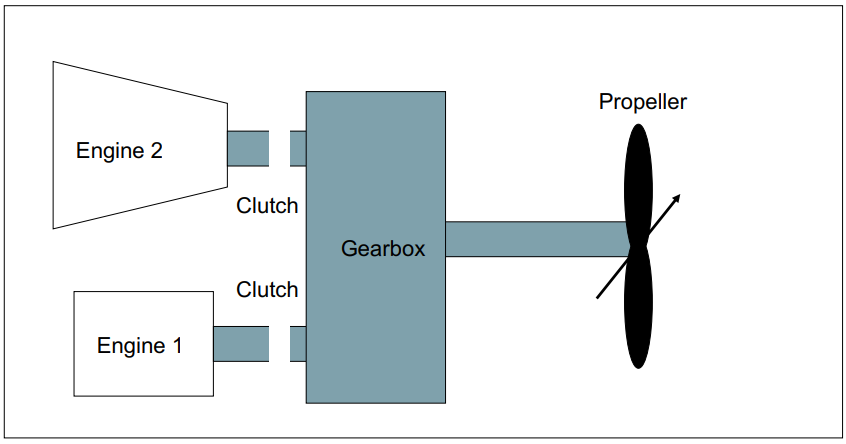
\includegraphics[width = 0.8\textwidth]{img/figure70.png}
    \caption{CODOG arrangement with CPP.}
\end{figure}

\begin{figure}[H]
    \centering
    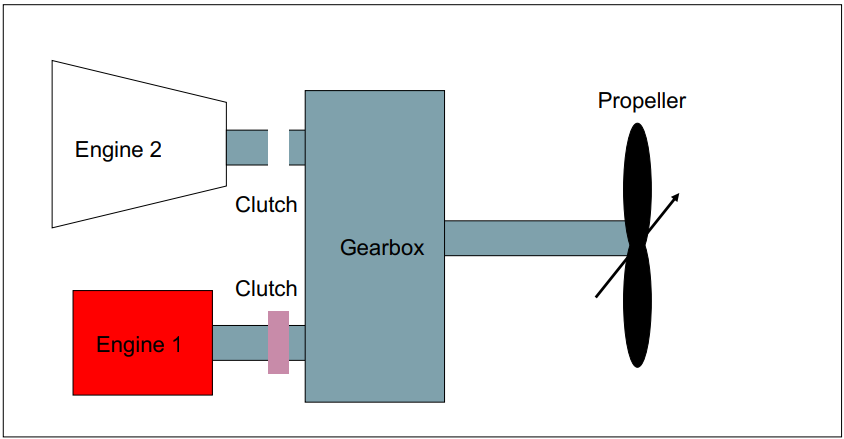
\includegraphics[width = 0.8\textwidth]{img/figure71.png}
    \caption{Engine 1 (low) power available for cruise speed.}
\end{figure}

\begin{figure}[H]
    \centering
    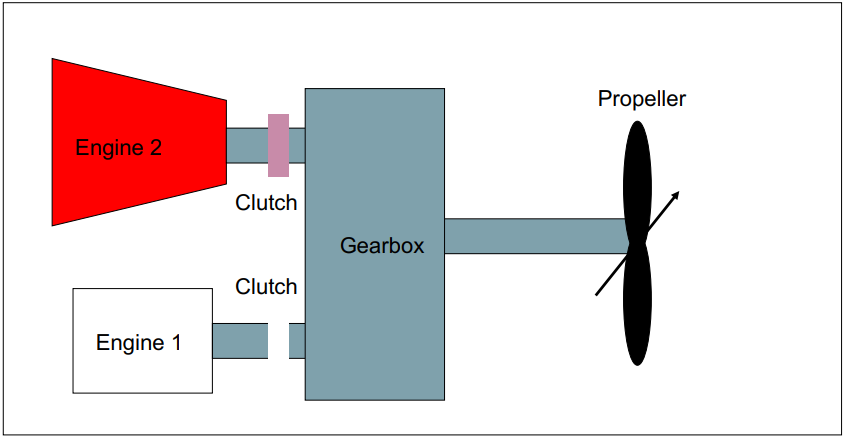
\includegraphics[width = 0.8\textwidth]{img/figure72.png}
    \caption{Engine 2 (large) power available for top speed.}
\end{figure}
\subsection{CODOG design issues}
\begin{itemize}
    \item Gas turbine supplied the power for maximum speed
    \item Diesel supplies the power for cruise speed (80\% MCR)
    \item The prime-movers are connected to the gearbox via clutches
    \item The engines work separately and not together
    \item The gearbox steps down the speeds of the prime-movers. (GT typically 3600-16000 \si{rpm}, propulsion diesels typically 400-1000 \si{rpm})
    \item The gearbox may also provide a reversing capability
    \item The propeller can be a fixed pitch or controllable pitch type (maximum shaft revolutions typically 150-200 \si{rpm})
\end{itemize}
\subsection{Alternative propulsion arrangements}
\begin{itemize}
    \item CODAG - combined diesel and gas turbine
    \item CODOD - combined diesel or diesel
    \item COGAG - combined gas turbine and gas turbine
    \item COGOG - combined gas turbine or gas turbine
    \item CODLAG - combined diesel electric and gas turbine
    \item COFCAG - combined fuel cell and gas turbine
    \item IFEP - integrated full electric propulsion
\end{itemize}
Note: first engine is cruise engine and second is t he sprint engine. AND / OR arrangements should be noted.
\section{Task 2}
A CODOG frigate has 3500 tonnes displacement. The specific delivered power coefficient ($C_D$) is 0.03 and may be assumed independent of ship's speed and power. The relationship can be expressed as:
\begin{gather}
    P_B = 1.04 \cdot C_D \cdot \rho^{0.33}\cdot \Delta^{0.67}\cdot V_S^3 \, (\si{\watt})
\end{gather}
\begin{itemize}
    \item $\rho$ is the seawater density \SI{1025}{\kilo\gram\per\meter\cubed}
    \item $\Delta$ is the displacement in \si{kg}
    \item $V$ is the speed of the advance in \si{\meter\per\second} (1 knot = \SI{0.514}{\meter\per\second})
\end{itemize}
The vessel has two shafts and a maximum speed of 30 knots and a cruising speed of 20 knots.

\textbf{\underline{Calculate the power rating of the engines}}.
\begin{gather}
    P_B = 1.04 \times 0.03 \times 1025^{0.33}\times \left(3500\times 10^3\right)^{0.67}\cdot V_S^3\\
    P_B = \left(7.5\times 10^3\right)\cdot V_S^3
\end{gather}
\textbf{Notes:}
\begin{enumerate}
    \item The relationship here is between engine break power and vessel speed of advance
    \item The relationship can be expressed as using effective power
\end{enumerate}
For the gas turbines here then $V_S = \SI{30}{knots} = \SI{15.43}{\meter\per\second}$.
\begin{itemize}
    \item $P_{B,GTS} = 7.5\times 10^3\times 15.43^3 = \SI{27500}{\kilo\watt}$
    \item Each gas turbine would be rated at \SI{13750}{\kilo\watt}
\end{itemize}
Gas turbines operating at flat out gives maximum power. For the diesel engines then $V_S = \SI{20}{knots} = \SI{10.29}{\meter\per\second}$.
\begin{itemize}
    \item $P_{B,DE} = 7.5\times 10^3 \times 10.29^3 = \SI{8200}{\kilo\watt}$
    \item Each diesel engine would be rated at \SI{5125}{\kilo\watt} assuming that they are rated at $0.8\times \textrm{MCR}$.
\end{itemize}
\textbf{Notes:}
\begin{enumerate}
    \item MCR - Maximum continuous rating
    \item \SI{1}{knot} = \SI{0.514}{\meter\per\second}
    \item We are assuming engines without NOx suppression
\end{enumerate}
\section{Task 3}
The frigate has an electrical service demand of 0.3 kW/(Tonne $\Delta$). Auxiliary power is to be supplied by two diesel generators such that in the normal condition they run at 80\% power. Generator efficiency is 95\%.

\textbf{\underline{Determine the size of the diesel generator sets}}.

Calculating the electrical load:
\begin{gather}
    0.3\times 3500 = \SI{1050}{\kilo\watt}
\end{gather}
Allowing for the generator efficiency of 95\%, then diesel engine output power must be \SI{1105}{\kilo\watt}. Two diesel engines have to operate at this mean load with 80\% power. Installed sets are therefore \SI{1380}{\kilo\watt}. Each diesel generator set will therefore be rated at \SI{690}{\kilo\watt} and operate at 80\% of MCR. Maximum electrical power available is:
\begin{gather}
    \frac{1105}{0.8} = \SI{1.381}{\mega\watt}
\end{gather}
\section{Task 4}
A journey is planned where at distance of 528 nautical miles must be covered in 24 hours. The captain is considering two alternatives to accomplish the mission:
\begin{enumerate}
    \item One speed of advance for the whole journey
    \item Fast sailing at 28 knots for 8 hours followed by the remaining time at a lower speed of advance
\end{enumerate}
For each option, you - the engineer, are to provide the captain with fuel consumption NOx emissions.
\begin{table}[H]
    \centering
    \begin{tabular}{@{}lllllll@{}}
        \toprule
        \textbf{\% Power} & \multicolumn{2}{l}{\textbf{Gas turbine}} & \multicolumn{2}{l}{\textbf{Main diesel}} & \multicolumn{2}{l}{\textbf{Diesel generator}}                                                                                           \\
                          & \textbf{SFC}                             & \textbf{NOXER}                           & \textbf{SFC}                                  & \textbf{NOXER}           & \textbf{SFC}                      & \textbf{NOXER}           \\
                          & \si{\gram\per\kilo\watt\per\hour}        & \si{\gram\per\kilo\gram}                 & \si{\gram\per\kilo\watt\per\hour}             & \si{\gram\per\kilo\gram} & \si{\gram\per\kilo\watt\per\hour} & \si{\gram\per\kilo\gram} \\
        \midrule
        25-34             & 350                                      & 5                                        & 250                                           & 74                       & 245                               & 74                       \\
        35-44             & 300                                      & 8.5                                      & 240                                           & 70                       & 240                               & 70                       \\
        45-54             & 280                                      & 9.5                                      & 230                                           & 66                       & 235                               & 65                       \\
        55-64             & 262                                      & 11                                       & 220                                           & 62                       & 230                               & 60                       \\
        65-74             & 258                                      & 12                                       & 208                                           & 58                       & 225                               & 51                       \\
        75-84             & 255                                      & 13                                       & 195                                           & 55                       & 220                               & 47                       \\
        85+               & 256                                      & 14                                       & 195                                           & 55                       & 220                               & 47                       \\
        \bottomrule
    \end{tabular}
    \caption{Data on fuel consumption NOx emissions - Task 4.}
    \label{task4Table}
\end{table}
\begin{itemize}
    \item SFC - specific fuel consumption
\end{itemize}
Speed of advance scenario 1:
\begin{gather}
    V_S = \frac{D}{T} = \frac{528}{24} = \SI{22}{knots} = \SI{11.31}{\meter\per\second}
\end{gather}
Speed of advance scenario 2. Phase 1:
\begin{gather}
    V_S = \SI{28}{knots} \textrm{ for 8 hours}\\
    D = 8\times 28 = \SI{224}{nm}
\end{gather}
Phase 2. Distance to cover in phase 2 is \SI{304}{nm}. Time to complete this distance is \SI{16}{\hour}.
\begin{gather}
    V_S = \frac{D}{T} = \SI{19}{knots} = \SI{9.77}{\meter\per\second}
\end{gather}
\subsection{Calculations - Scenario 1}
Calculate part load power for propulsion at 22 knots (\SI{11.31}{\meter\per\second}).
\begin{gather}
    P = 7.5 \times 10^3 \times 11.31^3 = \SI{10850}{\kilo\watt}
\end{gather}
Calculate this as a percentage of maximum output power. (note: $P_{B,GTS}$ is used here)
\begin{gather}
    \textrm{\% Power} = \frac{10850}{27500} = 39\%
\end{gather}
From Table \ref{task4Table}:
\begin{itemize}
    \item SFC: \SI{300}{\gram\per\kilo\watt\per\hour}
    \item NOXER: \SI{8.5}{\gram\per\kilo\gram}
\end{itemize}
Propulsion - calculate specific NOx emissions (SNE) (\si{\gram\per\kilo\watt\per\hour}):
\begin{align}
    \textrm{SNE} & = \textrm{NOXER} \times \textrm{SFC}                                   \\
    \textrm{SNE} & = 8.5\times \frac{300}{1000} = \SI{2.55}{\gram\per\kilo\watt\per\hour}
\end{align}
Propulsion - calculate fuel consumption:
\begin{gather}
    \textrm{mass/hour} = \textrm{SFC}\times P = 300 \times 10850 = \SI{3.26}{tonnes\per\hour}\\
    \textrm{Fuel consumed} = \textrm{mass/hour} \times T = 3.26 \times 24 = \SI{78.2}{tonnes}
\end{gather}
Propulsion - calculate NOx emissions:
\begin{gather}
    \textrm{Mass of NOx/hour} = \textrm{SNE}\times P = 2.55 \times 10850 = \SI{27.7}{\kilo\gram\per\hour}\\
    \textrm{NOx produced} = 27.7 \times 24 = \SI{665}{\kilo\gram}
\end{gather}
Calculate fuel consumption and NOx emissions for diesel generator sets.
\begin{itemize}
    \item Diesel generator are working at 80\% loading
    \item SFC = \SI{220}{\gram\per\kilo\watt\per\hour} (Table \ref{task4Table})
    \item NOXER = \SI{47}{\gram\per\kilo\gram} (Table \ref{task4Table})
\end{itemize}
Generation - calculate fuel consumption:
\begin{gather}
    \textrm{mass of fuel} = 220 \times 1105 \times 24 = \SI{5.8}{tonnes}
\end{gather}
Generation - calculate NOx emission:
\begin{gather}
    \textrm{mass of NOx} = 47 \times \frac{220}{1000} \times 1105 \times 24 = \SI{275}{\kilo\gram}
\end{gather}
Total fuel consumed (propulsion + generation):
\begin{gather}
    78.2+5.8=\SI{84}{tonnes}
\end{gather}
Total NOx emitted (propulsion + generation):
\begin{gather}
    665 + 275 =\SI{940}{\kilo\gram}
\end{gather}
\subsection{Calculations - Scenario 2}
First 8 hours at 28 knots (\SI{14.4}{\meter\per\second}):
\begin{gather}
    P = 7.5\times 10^3 \times 14.4^3 = \SI{22400}{\kilo\watt} \, (81\%)\\
    \textrm{SFC} = \SI{255}{\gram\per\kilo\watt\per\hour}\\
    \textrm{NOXER} = \SI{13}{\gram\per\kilo\gram}\\
    \textrm{SNE} = \textrm{NOXER}\times \textrm{SFC} = 13\times \frac{255}{1000} = \SI{3.22}{\gram\per\kilo\watt\per\hour}\\
    \textrm{mass of fuel used} = 255\times 22400 \times 8 = \SI{45.7}{tonnes}\\
    \textrm{NOx} = 3.22\times 22400\times 8 = \SI{595}{\kilo\gram}
\end{gather}
Last 16 hours at 19 knots (\SI{9.8}{\meter\per\second}):
\begin{gather}
    P = 7.5\times 10^3 \times 9.8^3 = \SI{7}{\mega\watt}\, (85\%)\\
    \textrm{SFC} = \SI{195}{\gram\per\kilo\watt\per\hour}\\
    \textrm{NOXER} = \SI{55}{\gram\per\kilo\gram}\\
    \textrm{SNE} = \textrm{NOXER} \times \textrm{SFC} = 55\times \frac{195}{1000} = \SI{10.7}{\gram\per\kilo\watt\hour}\\
    \textrm{mass of fuel used} = 195 \times 7000\times 16 = \SI{21.9}{tonnes}\\
    \textrm{NOx} = 10.7 \times 7000 \times 16 = \SI{1198}{\kilo\gram}
\end{gather}
Total fuel consumed (propulsion + generation):
\begin{gather}
    45.7 + 21.9 + 5.8 = \SI{73.4}{tonnes}
\end{gather}
Total NOx emitted (propulsion + generation):
\begin{gather}
    595 + 1198 + 275 = \SI{2068}{\kilo\gram}
\end{gather}
\subsection{Observations of study}
What is the difference in fuel consumption between 1 and 2?
\begin{quoting}
    \SI{10.6}{tonnes} i.e. 2 is 87\% of 1.
\end{quoting}
What vessel speed would give the worst fuel consumption?
\begin{quoting}
    GTs light load - 22 knots approximately
\end{quoting}
Which scenario has the best NOx performance and by how much?
\begin{quoting}
    \SI{1128}{\kilo\gram} less in favour of scenario 1
\end{quoting}
\subsubsection{A word on emissions!}
Carbon dioxide is dependent solely on fuel burnt i.e. the carbon factor of the fuel and the fuel consumption. For diesel the fuel consumption is approximately \SI{3.2}{tonnes} of carbon dioxide for \SI{1}{tonne} of fuel burnt. NOx is dependent on the combustion processes and in particular temperature and pressure. The higher the combustion pressure the more efficient the engine but more NOx produced. Sulphur emissions depends upon the amount of sulphur in the fuel. Particulates is dependent upon fuel quality and combustion processes.
\subsubsection{Carbon dioxide emissions}
Carbon dioxide emissions are directly related to fuel burnt regardless of how this is done whether in an internal combustion engine, gas turbine or boiler. \SI{1}{tonne} of distilled marine diesel fuel will emit 3.2 or more tonnes of CO2 depending upon fuel quality and lube oil consumption. We will use 3.2 for simplicity.
\begin{itemize}
    \item Scenario 1 produces: 84$\times$3.2 = 269 tonnes CO2
    \item Scenario 2 produces: 73.4$\times$3.2 = 234 tonnes CO2
\end{itemize}
\underline{Note the conflict}:
Burn less fuel and pollute with NOx more OR burn more fuel and pollute with NOx less\dots but CO2 more! In part this is why many diesel engines are being fitted with exhaust after treatment to eliminate (as much as possible, NOx).
\section{Task 5 (formative)}
Escorting the frigate is a sister ship (same displacement) which has an Integrated Full Electric Propulsion (IFEP) arrangement rather than the CODOG arrangement. The electrical propulsion system consists of generators, power converters and propulsion motors as seen on the next slide. The ship designer has selected the same prime-mover ratings for this design. Each gas turbine is rated at \SI{13750}{\kilo\watt} and each diesel rated at \SI{5815}{\kilo\watt} thereby providing engine compatibility across the fleet. The IFEP feeds both propulsion and service power loads. Because the diesels and gas turbines are operated along the generator line rather than the propulsion curve the data provided in the following slides should be used for NOXER values. Efficiency values of electrical machines are also provided to understand where losses occur.
\begin{figure}[H]
    \centering
    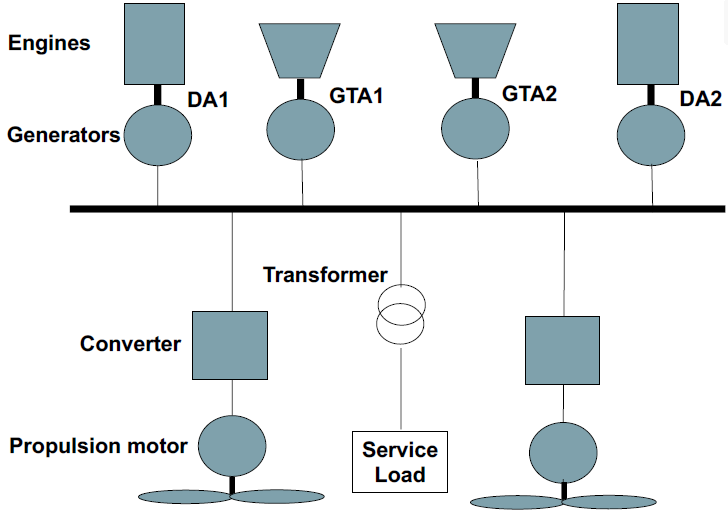
\includegraphics[width = 0.8\textwidth]{img/figure73.png}
    \caption{Task 5 Line diagram (use CODOG prime-movers).}
\end{figure}
\begin{table}[H]
    \centering
    \begin{tabular}{@{}lll@{}}
        \toprule
        \textbf{Power input} & \textbf{Generator (constant N)} & \textbf{Motor (Variable N)} \\
        \midrule
        0\%                  & 0\%                             & 0\%                         \\
        20\%                 & 65\%                            & 60\%                        \\
        40\%                 & 85\%                            & 80\%                        \\
        60\%                 & 90\%                            & 90\%                        \\
        80\%                 & 95\%                            & 96\%                        \\
        100\%                & 95\%                            & 96\%                        \\
        \bottomrule
    \end{tabular}
    \caption{Efficiency of generators and motors}
\end{table}
Power converters (AC:DC:AC): can be considered to be 95\% across the full power range. Transformer efficiency: 95\%.
\begin{table}[H]
    \centering
    \begin{tabular}{@{}lllll@{}}
        \toprule
        \textbf{\% Power} & \multicolumn{2}{l}{\textbf{Gas turbine}} & \multicolumn{2}{l}{\textbf{Diesel generator}}                                                                \\
                          & \textbf{SFC}                             & \textbf{NOXER}                                & \textbf{SFC}                      & \textbf{NOXER}           \\
                          & \si{\gram\per\kilo\watt\per\hour}        & \si{\gram\per\kilo\gram}                      & \si{\gram\per\kilo\watt\per\hour} & \si{\gram\per\kilo\gram} \\
        \midrule
        25-34             & 330                                      & 5                                             & 245                               & 74                       \\
        35-44             & 290                                      & 8.5                                           & 240                               & 70                       \\
        45-54             & 275                                      & 9.5                                           & 235                               & 65                       \\
        55-64             & 259                                      & 11                                            & 230                               & 60                       \\
        65-74             & 257                                      & 12                                            & 225                               & 51                       \\
        75-84             & 255                                      & 13                                            & 220                               & 47                       \\
        85+               & 255                                      & 14                                            & 220                               & 47                       \\
        \bottomrule
    \end{tabular}
    \caption{Data on fuel consumption NOx emissions - Task 5.}
    \label{task5Table}
\end{table}
\subsection{Task A}
\begin{enumerate}
    \item Suggest the required electrical equipment ratings i.e. \si{\kilo\watt} ratings of generator, converter and motor based on given installed prime-mover powers for the electric frigate
    \item Determine for your design the fuel consumptions and exhaust gas emissions for scenario 1 and scenario 2 for the electric frigate
    \item Compare and contrast between CODOG and IFEP arrangements (use tables and graphs)
          \begin{itemize}
              \item Compare maximum possible speed of the two vessels
              \item Ideal cruise speeds of the two vessels
              \item Running hours of the engines for the two scenarios
              \item The likely cooling requirements for each vessel's propulsion system
          \end{itemize}
\end{enumerate}
\subsection{Task B}
Using library resources and web resources, summarise an investigation into commercial shipping use of electrical propulsion today. Discuss at least three key technologies that are under development.